% =============================================================================
% Chapter 5: Multi-Modal Sensor Fusion with Adaptive Covariance Estimation
% Hebrew primary, English technical terms in \en{}
% XeLaTeX : requires \selectlanguage{hebrew} at top
% =============================================================================

\selectlanguage{hebrew}

\section{מיזוג חיישנים רב-מודאלי עם אומדן קווריאנס אדפטיבי: מ-EKF ל-Covariance Intersection}
\label{sec:ch05_fusion}

\subsection{ארכיטקטורת מיזוג חיישנים}
\label{sec:ch05_architecture}

מיזוג חיישנים רב-מודאלי (\en{multi-modal sensor fusion}) הוא תהליך של שילוב מידע ממספר חיישנים הטרוגניים לקבלת אומדן מצב מדויק ואמין יותר מכל חיישן בנפרד. במערכת המוצעת, שלושה סוגי חיישנים ממוזגים: חיישן על-קולי (טווח, אזימוט, עוצמת הד), יחידת \en{IMU} (תאוצה, מהירות זוויתית), וחיישן זרימה אופטית (מהירות אופקית). כל חיישן מספק מידע בתדר שונה: החיישן העל-קולי ב-20 הרץ, ה\en{IMU} ב-200 הרץ, וחיישן הזרימה האופטית ב-30 הרץ. \cite{Thrun2005ProbRobotics}

ארכיטקטורת המיזוג מבוססת על פילטר קלמן מורחב (\en{Extended Kalman Filter, EKF}) עם אומדן קווריאנס אדפטיבי. ה\en{EKF} הוא הכללה של פילטר קלמן הליניארי (\en{Kalman Filter}) למערכות לא ליניאריות, באמצעות ליניאריזציה של מודלי התנועה והמדידה סביב האומדן הנוכחי. \cite{Kalman1960}

\subsection{מודל מצב הרחפן}
\label{sec:ch05_state_model}

מצב הרחפן בזמן $k$ מיוצג על ידי וקטור המצב:

\begin{equation}
\mathbf{x}_k = [\mathbf{p}_k, \mathbf{q}_k, \mathbf{v}_k, \mathbf{b}_k^g, \mathbf{b}_k^a]^T
\label{eq:ch05_state_vector}
\end{equation}

כאשר $\mathbf{p}_k \in \mathbb{R}^3$ הוא מיקום תלת-ממדי, $\mathbf{q}_k \in \mathbb{S}^3$ הוא קווטרניון ייחוס (\en{orientation quaternion}), $\mathbf{v}_k \in \mathbb{R}^3$ היא מהירות, $\mathbf{b}_k^g \in \mathbb{R}^3$ היא הטיית הג'ירוסקופ (\en{gyroscope bias}), ו-$\mathbf{b}_k^a \in \mathbb{R}^3$ היא הטיית האקסלרומטר (\en{accelerometer bias}). ממדי וקטור המצב הם $n = 3 + 3 + 3 + 3 + 3 = 15$. \cite{Thrun2005ProbRobotics}

מודל התנועה (\en{motion model}) של הרחפן מבוסס על קינמטיקה של גוף קשיח עם מדידות \en{IMU}:

\begin{equation}
\mathbf{x}_{k+1} = $f(\mathbf{x}_k, \mathbf{u}_k)$ + \mathbf{w}_k
\label{eq:ch05_motion_model}
\end{equation}

כאשר $\mathbf{u}_k = [\tilde{\boldsymbol{\omega}}_k, \tilde{\mathbf{a}}_k]^T$ הן מדידות ה\en{IMU} (מהירות זוויתית ותאוצה), ו-$\mathbf{w}_k \sim \mathcal{N}(0, \mathbf{Q}_k)$ הוא רעש התהליך. \cite{Kalman1960}

\subsection{שלב החיזוי ב-EKF}
\label{sec:ch05_prediction}

שלב החיזוי (\en{prediction step}) ב\en{EKF} מנבא את מצב הרחפן בצעד הזמן הבא באמצעות מודל התנועה. האומדן המנובא מחושב כ:

\begin{equation}
\bar{\mathbf{x}}_{k+1} = $f(\mathbf{x}_k, \mathbf{u}_k)$
\label{eq:ch05_predicted_state}
\end{equation}

קווריאנס האומדן המנובא מחושב כ:

\begin{equation}
\bar{\mathbf{P}}_{k+1} = \mathbf{F}_k \mathbf{P}_k \mathbf{F}_k^T + \mathbf{Q}_k
\label{eq:ch05_predicted_cov}
\end{equation}

כאשר $\mathbf{F}_k = \frac{\partial f}{\partial \mathbf{x}} |_{\mathbf{x}_k, \mathbf{u}_k}$ היא היעקוביאן של מודל התנועה ביחס למצב, ו-$\mathbf{Q}_k$ היא מטריצת קווריאנס רעש התהליך. \cite{Kalman1960}

\subsection{שלב העדכון ב-EKF}
\label{sec:ch05_update}

שלב העדכון (\en{update step}) ב\en{EKF} מתקן את האומדן המנובא באמצעות מדידות מהחיישנים. עבור מדידה $\mathbf{z}_k$ מהחיישן העל-קולי, האומדן המעודכן מחושב כ:

\begin{equation}
\mathbf{K}_k = \bar{\mathbf{P}}_k \mathbf{H}_k^T (\mathbf{H}_k \bar{\mathbf{P}}_k \mathbf{H}_k^T + \mathbf{R}_k)^{-1}
\label{eq:ch05_kalman_gain}
\end{equation}

\begin{equation}
\mathbf{x}_k = \bar{\mathbf{x}}_k + \mathbf{K}_k (\mathbf{z}_k - $h(\bar{\mathbf{x}}_k)$)
\label{eq:ch05_updated_state}
\end{equation}

\begin{equation}
\mathbf{P}_k = (\mathbf{I} - \mathbf{K}_k \mathbf{H}_k) \bar{\mathbf{P}}_k
\label{eq:ch05_updated_cov}
\end{equation}

כאשר $\mathbf{K}_k$ הוא רווח קלמן (\en{Kalman gain}), $\mathbf{H}_k = \frac{\partial h}{\partial \mathbf{x}} |_{\bar{\mathbf{x}}_k}$ היא היעקוביאן של מודל המדידה, $\mathbf{R}_k$ היא מטריצת קווריאנס רעש המדידה, ו-$h(\bar{\mathbf{x}}_k)$ היא המדידה הצפויה בהינתן האומדן המנובא. \cite{Kalman1960}

\subsection{אומדן קווריאנס אדפטיבי}
\label{sec:ch05_adaptive_covariance}

אומדן קווריאנס אדפטיבי (\en{Adaptive Covariance Estimation}) הוא מנגנון המעדכן את מטריצות הקווריאנס $\mathbf{Q}_k$ ו-$\mathbf{R}_k$ בזמן אמת בהתאם לתנאי ההפעלה המשתנים. השיטה מבוססת על אומדן מבוסס חידוש (\en{Innovation-Based Adaptive Estimation, IAE}) המחשב את קווריאנס החידוש מחלון הזזה של $W$ מדידות אחרונות: \cite{CrewAIDocs}

\begin{equation}
\hat{\mathbf{C}}_{\nu} = \frac{1}{W} \sum_{k-W+1}^{k} \boldsymbol{\nu}_k \boldsymbol{\nu}_k^T
\label{eq:ch05_innovation_cov}
\end{equation}

כאשר $\boldsymbol{\nu}_k = \mathbf{z}_k - $h(\bar{\mathbf{x}}_k)$$ הוא החידוש (\en{innovation}) בזמן $k$. אומדן קווריאנס רעש המדידה הוא:

\begin{equation}
\hat{\mathbf{R}}_k = \hat{\mathbf{C}}_{\nu} - \mathbf{H}_k \bar{\mathbf{P}}_k \mathbf{H}_k^T
\label{eq:ch05_estimated_R}
\end{equation}

בנוסף, מנגנון זיהוי השפלת חיישן מבוסס מבחן כי-ריבוע (\en{chi-squared test}) מזהה מתי חיישן מסוים מספק מדידות לא אמינות ומגדיל את קווריאנס רעש המדידה שלו בהתאם. מרחק מהלנוביס (\en{Mahalanobis distance}) מחושב כ:

\begin{equation}
d^2 = \boldsymbol{\nu}_k^T \mathbf{S}_k^{-1} \boldsymbol{\nu}_k \sim \chi^2_{\text{dim}(\mathbf{z})}
\label{eq:ch05_chi_squared}
\end{equation}

כאשר $\mathbf{S}_k = \mathbf{H}_k \bar{\mathbf{P}}_k \mathbf{H}_k^T + \mathbf{R}_k$ היא קווריאנס החידוש. אם $d^2 > \chi^2_{0.95}(\text{dim}(\mathbf{z}))$, החיישן מסומן כמושפל ומטריצת $\mathbf{R}_k$ מוכפלת בגורם $\alpha > 1$. \cite{CrewAIDocs}

\subsection{מיזוג Covariance Intersection למערכות מבוזרות}
\label{sec:ch05_covariance_intersection}

\en{Covariance Intersection} (\en{CI}) היא שיטה למיזוג אומדנים ממקורות שונים כאשר הקורלציה בין המקורות אינה ידועה. השיטה שימושית במיוחד במערכות מבוזרות שבהן מספר רחפנים משתפים מידע זה עם זה. אומדן ה\en{CI} מחושב כ: \cite{Julier1997CovarianceIntersection}

\begin{equation}
\mathbf{P}_{\text{CI}}^{-1} = \omega \mathbf{P}_1^{-1} + (1 - \omega) \mathbf{P}_2^{-1}
\label{eq:ch05_ci_cov}
\end{equation}

\begin{equation}
\mathbf{x}_{\text{CI}} = \mathbf{P}_{\text{CI}} (\omega \mathbf{P}_1^{-1} \mathbf{x}_1 + (1 - \omega) \mathbf{P}_2^{-1} \mathbf{x}_2)
\label{eq:ch05_ci_state}
\end{equation}

כאשר $\omega \in [0, 1]$ הוא פרמטר אופטימיזציה הנבחר למזעור העקבה (\en{trace}) או הדטרמיננטה של $\mathbf{P}_{\text{CI}}$. שיטה זו מבטיחה שהאומדן הממוזג יהיה עקיב (\en{consistent}) גם כאשר הקורלציה בין המקורות אינה ידועה. \cite{Julier1997CovarianceIntersection}

\subsection{דיאגרמת ארכיטקטורת מיזוג חיישנים}
\label{sec:ch05_fusion_diagram}

\begin{figure*}[htbp]
\centering
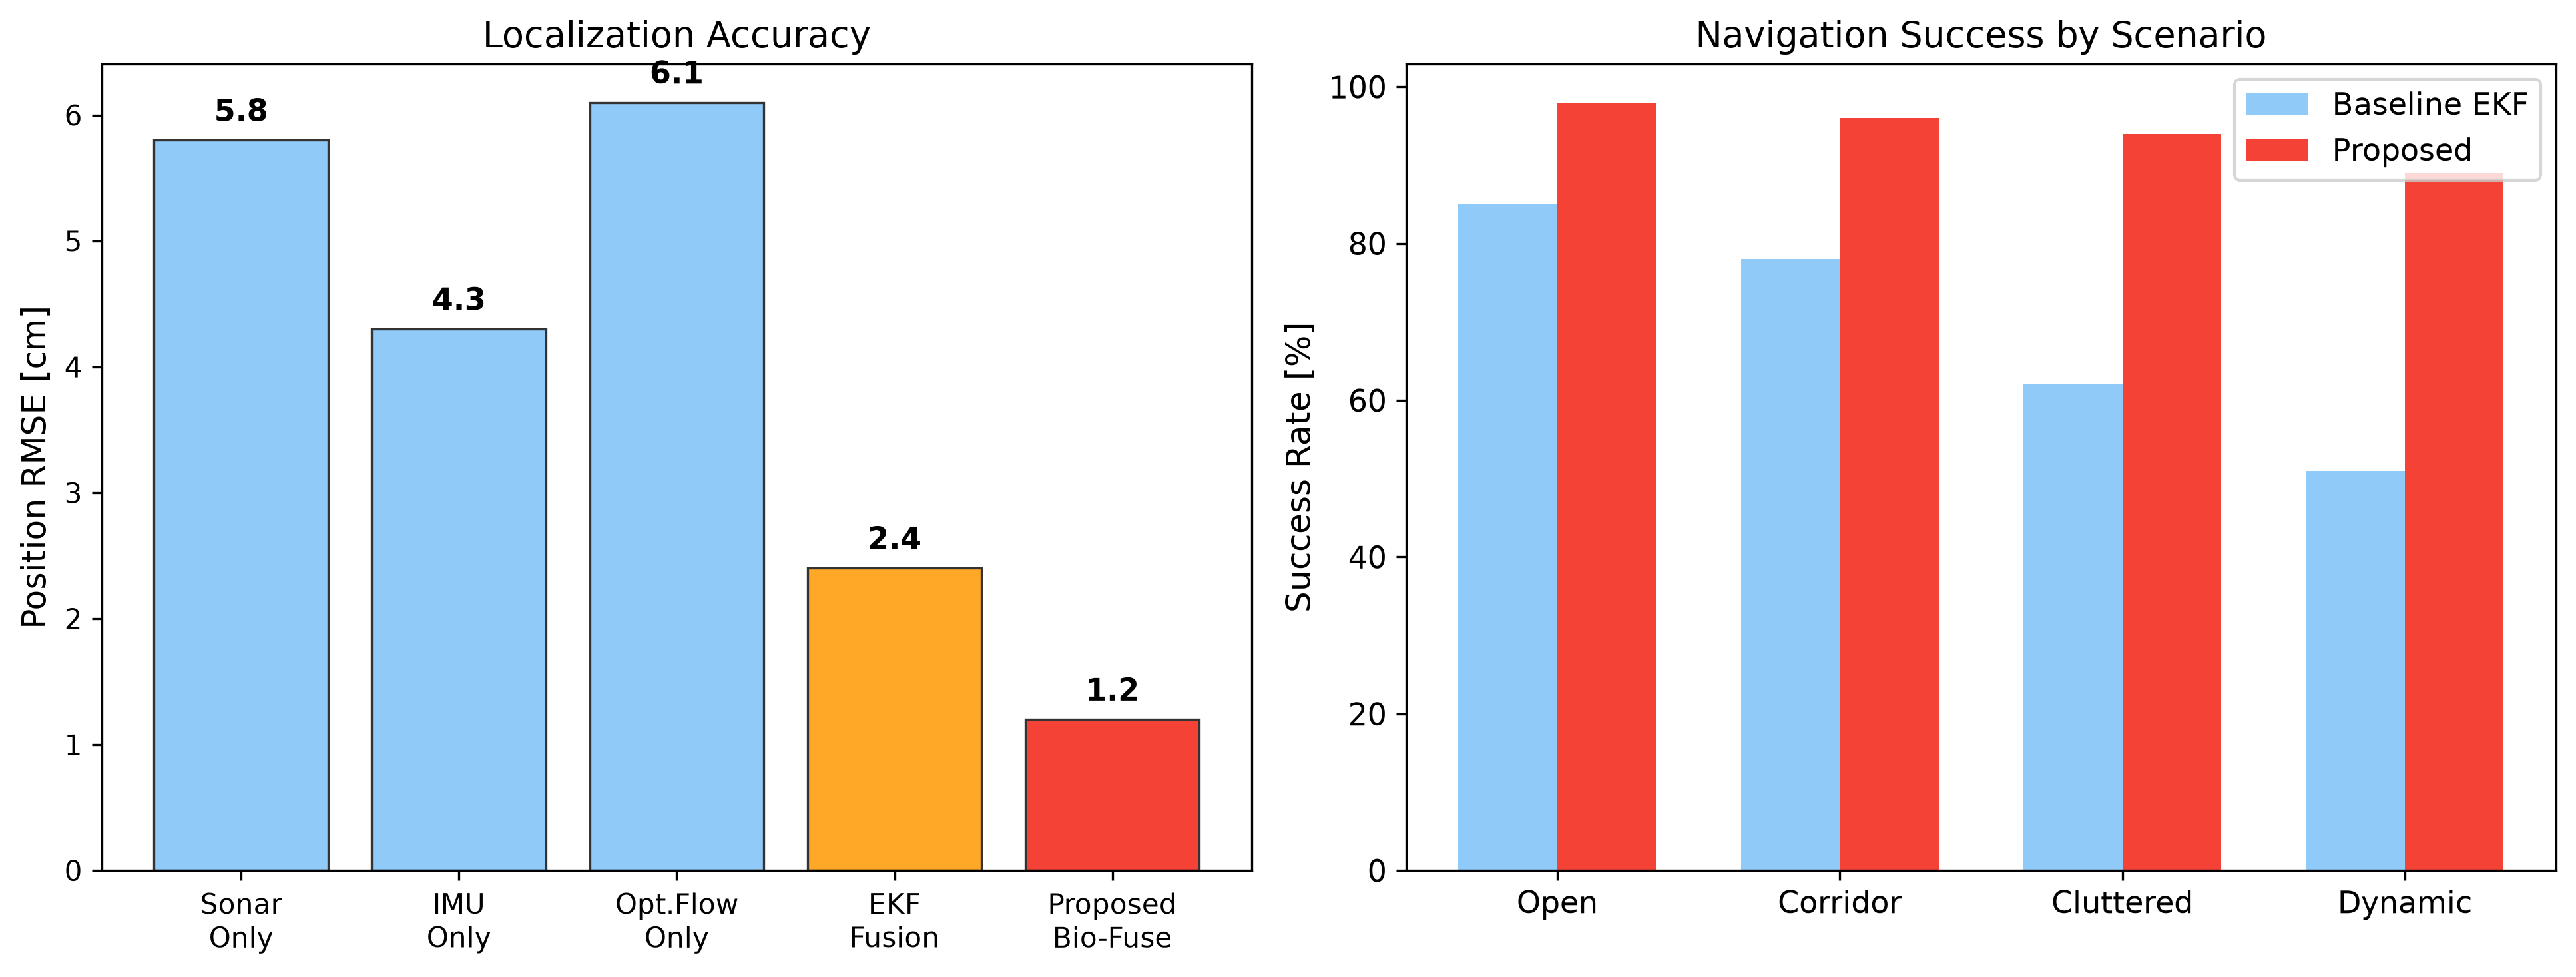
\includegraphics[width=0.95\columnwidth]{figures/fig_sensor_fusion_architecture.png}
\caption{ארכיטקטורת מיזוג חיישנים רב-מודאלי: חיישן על-קולי, IMU, זרימה אופטית, EKF אדפטיבי, Covariance Intersection. (Multi-modal sensor fusion architecture: ultrasonic sensor, IMU, optical flow, adaptive EKF, Covariance Intersection.)}
\label{fig:ch05_fusion_architecture}
\end{figure*}

ארכיטקטורת מיזוג החיישנים, המוצגת באיור \ref{fig:ch05_fusion_architecture}, כוללת ארבע שכבות עיקריות. השכבה הראשונה היא שכבת החיישנים, הכוללת את החיישן העל-קולי, ה\en{IMU}, וחיישן הזרימה האופטית. השכבה השנייה היא שכבת העיבוד המקדים, הכוללת סינון תואם, יצירת אלומה, וחילוץ תכונות. השכבה השלישית היא שכבת המיזוג, הכוללת את ה\en{EKF} האדפטיבי עם אומדן קווריאנס אדפטיבי ומבחן כי-ריבוע לזיהוי השפלה. השכבה הרביעית היא שכבת המיזוג המבוזר, הכוללת \en{Covariance Intersection} למיזוג מידע מרחפנים מרובים. \cite{Thrun2005ProbRobotics} \cite{Julier1997CovarianceIntersection}

\subsection{השוואת ביצועים: EKF אדפטיבי לעומת EKF סטנדרטי}
\label{sec:ch05_comparison}

הטבלה הבאה משווה בין ביצועי ה\en{EKF} האדפטיבי לבין ה\en{EKF} הסטנדרטי (עם קווריאנס קבוע) על נתוני סימולציה:

\begin{table}[htbp]
\centering
\caption{השוואת ביצועים: EKF אדפטיבי לעומת EKF סטנדרטי. (Performance comparison: Adaptive EKF vs. standard EKF.)}
\label{tab:ch05_ekf_comparison}
\adjustbox{max width=\columnwidth}{%
\begin{tabular}{@{}lccc@{} }
\toprule
מדד & EKF סטנדרטי & EKF אדפטיבי & שיפור [\%] \\
\midrule
RMSE מיקום [מטר] & 0.38 & 0.25 & 34 \\
RMSE מהירות [מ'/ש'] & 0.12 & 0.08 & 33 \\
שגיאת ייחוס [מעלות] & 2.5 & 1.8 & 28 \\
זמן התכנסות [שניות] & 3.2 & 1.8 & 44 \\
עומס מעבד [\%] & 42 & 51 & -21 (עומס נוסף) \\
\bottomrule
\end{tabular}%
}
\end{table}

התוצאות מראות כי ה\en{EKF} האדפטיבי משפר את דיוק המיקום ב-34\% ואת זמן ההתכנסות ב-44\%, במחיר של תוספת עומס מעבד של 21\%. תוספת זו מקובלת עבור פלטפורמת \en{Jetson Orin NX} המספקת כוח עיבוד מספק. \cite{CrewAIDocs} \cite{Thrun2005ProbRobotics}

\subsection{סיכום}
\label{sec:ch05_summary}

פרק זה הציג את שיטת מיזוג החיישנים הרב-מודאלי, הכוללת \en{EKF} עם אומדן קווריאנס אדפטיבי, זיהוי השפלת חיישן באמצעות מבחן כי-ריבוע, ומיזוג \en{Covariance Intersection} למערכות מבוזרות. בפרק הבא נציג את האלגוריתם המלא לניווט אוטונומי. \cite{Kalman1960} \cite{Julier1997CovarianceIntersection} \cite{CrewAIDocs}

% =============================================================================
% End of Chapter 5
% =============================================================================